%=========================================================================
% (c) 2014, 2015 Josef Lusticky

\chapter{40 Gigabit Ethernet}

The growth of Ethernet from 10 Mbit/s to 10 Gbit/s has surpassed the growth of microprocessor performance.
A fundamental obstacle to improving network performance is that servers were designed for computing rather than input and output (I/O).
The Internet revolution has drastically changed server requirements,
and I/O is becoming a major bottleneck in delivering high-speed computing.
The main reason for the bottleneck is the TCP/IP stack being processed at a rate less than the network speed.
The processing of TCP/IP over Ethernet is traditionally accomplished by software running on the CPUs of the server.
As network connections scale beyond Gigabit Ethernet speeds,
the CPU becomes burdened with the large amount of TCP/IP protocol processing required.
Reassembling out-of-order packets, resource-intensive memory copies, and interrupts put a tremendous load on the host CPU.
In high-speed networks, the CPU has to dedicate more processing to handle the network traffic than to the applications it is running.
A rough estimate of the CPU processing required to handle a given Ethernet link speed is,
for every one bit per second of network data processed, one hertz of CPU processing is required.
This general rule of thumb was first stated by PC Magazine in the mid 1990’s, and is still used as a rule of thumb today.
http://www.10gea.org/whitepapers/tcpip-offload-engine-toe/




Previous Ethernet versions could use standard Cat 6 copper cable and RJ-45 connectors , %~\cite{10gbase-t}
whereas 40 Gigabit runs on Quad Small Form Factor Pluggable (QSPF) - a high-density fiber connector with 12 strands of fiber.

http://searchdatacenter.techtarget.com/feature/40-GbE-technology-Hurry-up-and-wait
Unlike standard two-strand fiber connections, it isn’t “field terminated,” meaning that an electrician can’t hook up a QSFP connector on site. Data center managers need to determine their cabling lengths in advance and preorder custom cables that are manufactured with the connectors already attached.


The channel layout is shown in figure~\ref{fig:40gbit-ethernet-layout}.

\begin{figure}
	\centering
	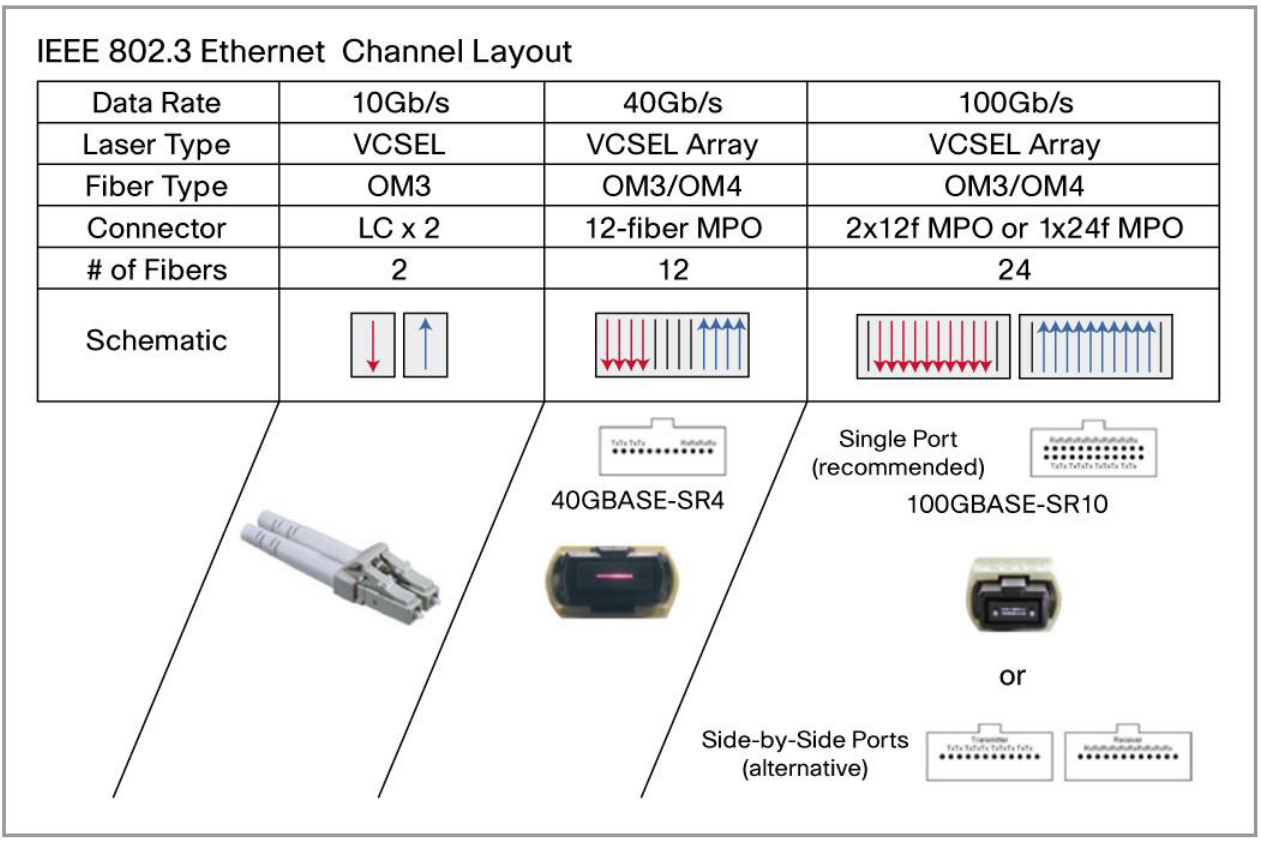
\includegraphics[width=13cm,keepaspectratio]{fig/ethernet-layout.pdf}
	\caption{IEEE 802.3 Ethernet Channel Layout (source: Cisco Systems Inc.)}
	\label{fig:40gbit-ethernet-layout}
	\bigskip
\end{figure}

40Gbit Ethernet is still Etherneth underneath - it is an old technology with a lot of compatibility issues for high speed networking.
The biggest of them being the 1500-byte maximum transfer unit (MTU).
There are some extensions to transfer larger frames, known as Jumbo frames,
but IEEE has determined they will not support or define Jumbo frames due to concerns around vendor and equipment interoperability.

http://www.ethernetalliance.org/wp-content/uploads/2011/10/EA-Ethernet-Jumbo-Frames-v0-1.pdf


a 10G network link running at full speed will be transferring over 700 000 packets per seconds

Most connections of interest go across the Internet, and those are all bound by the lowest MTU in the entire path
and sometimes that MTU is even less than 1500 bytes.
So, while Jumbo frames might work well for local networks, there is still a limit of 1500 bytes on the wider Internet.
https://lwn.net/Articles/358910/
